\documentclass[11pt,a4paper]{jsarticle}
%
\usepackage{amsmath}
\usepackage{algorithm}
\usepackage{algorithmic}
\usepackage{bm}
\usepackage{color}
\usepackage[dvipdfmx]{graphicx}
\usepackage{multicol}
\usepackage[psamsfonts]{amssymb}
\usepackage{url}
\usepackage{listings,jlisting}
\usepackage[dvipdfmx]{hyperref}
\usepackage{pxjahyper}

\lstset{
	%プログラム言語(複数の言語に対応,C,C++も可)
 	language = Python,
 	%背景色と透過度
 	backgroundcolor={\color[gray]{.90}},
 	%枠外に行った時の自動改行
 	breaklines = true,
 	%自動改行後のインデント量(デフォルトでは20[pt])	
 	breakindent = 10pt,
 	%標準の書体
 	basicstyle = \ttfamily\scriptsize,
 	%コメントの書体
 	commentstyle = {\itshape \color[cmyk]{1,0.4,1,0}},
 	%関数名等の色の設定
 	classoffset = 0,
 	%キーワード(int, ifなど)の書体
 	keywordstyle = {\bfseries \color[cmyk]{0,1,0,0}},
 	%表示する文字の書体
 	stringstyle = {\ttfamily \color[rgb]{0,0,1}},
 	%枠 "t"は上に線を記載, "T"は上に二重線を記載
	%他オプション:leftline,topline,bottomline,lines,single,shadowbox
 	frame = TBrl,
 	%frameまでの間隔(行番号とプログラムの間)
 	framesep = 5pt,
 	%行番号の位置
 	numbers = left,
	%行番号の間隔
 	stepnumber = 1,
	%行番号の書体
 	numberstyle = \tiny,
	%タブの大きさ
 	tabsize = 2,
 	%キャプションの場所("tb"ならば上下両方に記載)
 	captionpos = t
}

%
%\setlength{\textwidth}{\fullwidth}
%\setlength{\textheight}{40\baselineskip}
% \addtolength{\textheight}{\topskip}
% \setlength{\voffset}{-0.2in}
% \setlength{\topmargin}{7mm}
% \addtolength{\topmargin}{-0.75in}
% \setlength{\oddsidemargin}{14mm}
% \addtolength{\oddsidemargin}{-1in}
% \setlength{\evensidemargin}{14mm}
% \addtolength{\evensidemargin}{-1in}
% \setlength{\textwidth}{170mm}
% \setlength{\textheight}{256mm}
% \setlength{\headsep}{0mm}
% \setlength{\headheight}{0mm}
% \setlength{\topskip}{0mm}

%
%%%%%%%%%%%%%%%%%%%%%%%%%%%%%%%%%%%%%%%%%%%%%%%%%%%%%%%%%%%%%%%%%%%%%%%%%%%%%%%%
%
\title{2020年度 Computer Vision\\最終レポート}
\author{慶應義塾大学 理工学研究科 専攻 修士1年 佐久間拓哉 (82019167)}
\date{\today}

\begin{document}
\maketitle
%
%%%%%%%%%%%%%%%%%%%%%%%%%%%%%%%%%%%%%%%%%%%%%%%%%%%%%%%%%%%%%%%%%%%%%%%%%%%%%%%%
%
\section{序論・問題文}
本レポートは「2D match move/augmented reality」を選択した。

近年、スポーツに使用されるスタジアムのバックネット広告に、
バーチャル広告が採用されているケースがある。
例えば2018年のボルシア・ドルトムントではビッチわきの広告版にこの技術を採用し、ヨーロッパやアメリカ、アジアそれぞれの試合中継で異なる広告を表示することで広告板を増やすことなく広告スペースを拡大することに成功している\cite{t}。

本レポートではこのバーチャル広告のベースとなる技術を実装する。
具体的には画像のワーピング、特徴量抽出及びマッチング、ホモグラフィ行列の算出を組み合わせて、対象画像の一部を差し替える。

以降の
\section{実装詳細}
問題の全体像を以下の図に示す。まず、図\ref{}(a)の部分画像ABCD(テンプレート画像)とマッチする部分画像EFGH(適用画像)を図中(c)から探索する。その後図中(b)の差し替え先画像から差し替え画像へのホモグラフィ行列を計算し、ワーピング処理によって差し替えを行う。

本レポートでは頂点ABCDの選定は手動で行うが、頂点EFGHは明示的に選択せず、特徴量マッチングによって暗黙的に行う。この場合、差し替え先画像から適用画像へのホモグラフィ行列は、各ピクセルの対応が分からないため、直接求めることはできない。そこで、テンプレート画像と差し替え先画像の画像サイズを一致させてから、テンプレート画像と適用画像との特徴量マッチングを行うことで、ここから求められるテンプレート画像から適用画像へのホモグラフィ行列が差し替え先画像から適用画像へのホモグラフィ行列に一致する。
このようにして各ピクセルの変換方法が求められるため画像を置換できる。

本章では、各操作の詳細アルゴリズム及び実装を述べる。

\subsection{実行環境}
本レポートは次の実行環境で動作させている。
\begin{itemize}
    \item Python 3.7
    \item kivy 1.11.1
    \item OpenCV-python 3.4.2.16
    \item Numpy 1.19.0
\end{itemize}



\subsection{テンプレート画像と差し替え先画像の画像サイズ}
本問題では図\ref{}(a)の頂点ABCDには任意性があるため、単純なリサイズ処理ではテンプレート画像と差し替え先画像のサイズを一致させることができない。
本レポートではワーピング処理によって頂点ABCDを矩形に変換する。
変換によって画像にピクセルの抜けが生じないようにするためInverse warpingを実装する。
具体的には以下の図\ref{}に示す、
四角形MNOP内の任意の点$(x_1, y_1)$から四角形IJKLの対応する点$(x_0, y_0)$を求める。
$(x_1, y_1)$から辺MNへの距離及び垂線の足をそれぞれ$d_MN$及び$\bm{}$


ワーピング処理の具体的な実装は以下のプログラム\ref{}に示す。




なお、一致させる画像サイズの決め方は次の二種類の方法が考えられる。
\begin{itemize}
    \item 差し替え先画像の高さ・幅に合わせる
    \item テンプレート画像の高さ・幅に合わせる
\end{itemize}
前者については、差し替え先画像は必ず長方形の形をしているため、簡単に高さや幅を取得することができる。


\subsection{マッチングアルゴリズム}
マッチングアルゴリズムには様々な手法が提案されているが、
本レポートではテンプレートマッチング及び特徴点マッチングをそれぞれ使用した。

\subsubsection{テンプレートマッチング}
テンプレートマッチングは画像の画素値そのものを特徴として扱うパターンマッチングの一種である\ref{}。
この手法では特徴となる画素値をテンプレートとして用意しておき、SSDを始めとする類似度を使用してマッチングを行う\ref{}。

本問題においても予めテンプレート画像は用意しておくが、
サイズが大きいため、精度が低下してしまうことが予想される。
さらに根本的な問題として、テンプレートマッチングでは各ピクセルの対応が取れるわけではなく、
一致する領域が得られるに過ぎないため、本問題の目的には合致しない。

そこで、本レポートではハリスのコーナー検出\ref{}を利用して特徴点を検出した後、
その点を中心とした部分画像をテンプレートとしてマッチングを行う。


\section{評価及び考察}\label{sec:eval}
本章では作成したアプリケーションの検出精度や実行速度を測り、
アプリケーションの実用性を評価する。
本評価で使用するテンプレート画像及び差し替え先画像を図\ref{fig:data}に示す。
なお、適用先画像については特に言及しない限り、
本レポートに添付した「target.mov」を使用する。
\begin{figure}[h]
    \centering
    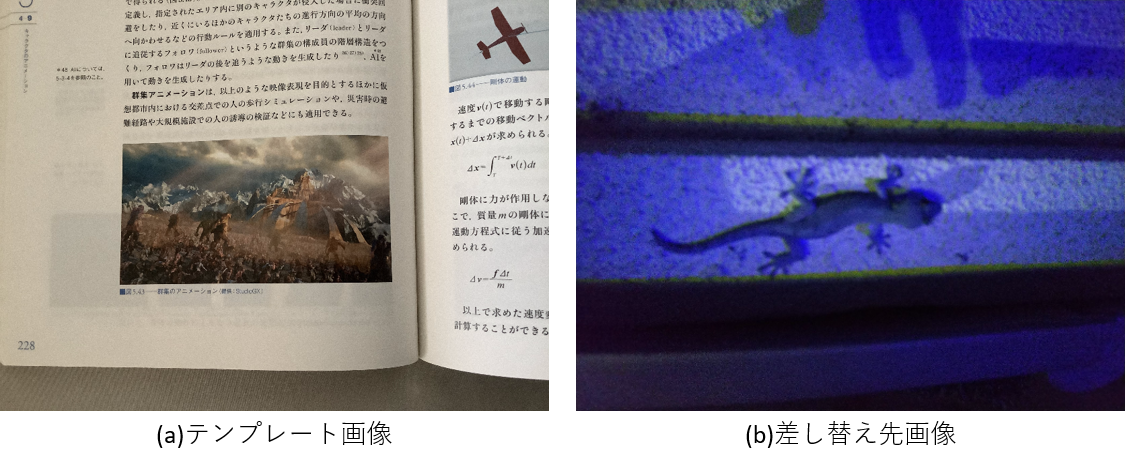
\includegraphics[width=1\linewidth]{fig/data.png}
    \caption{評価データ}
    \label{fig:data}
\end{figure}
なお、テンプレート画像については無駄な領域を省くために図\ref{fig:clip}で示されるように、
アプリケーション内でユーザが領域を選択しクリッピングしておく。
\begin{figure}[h]
    \centering
    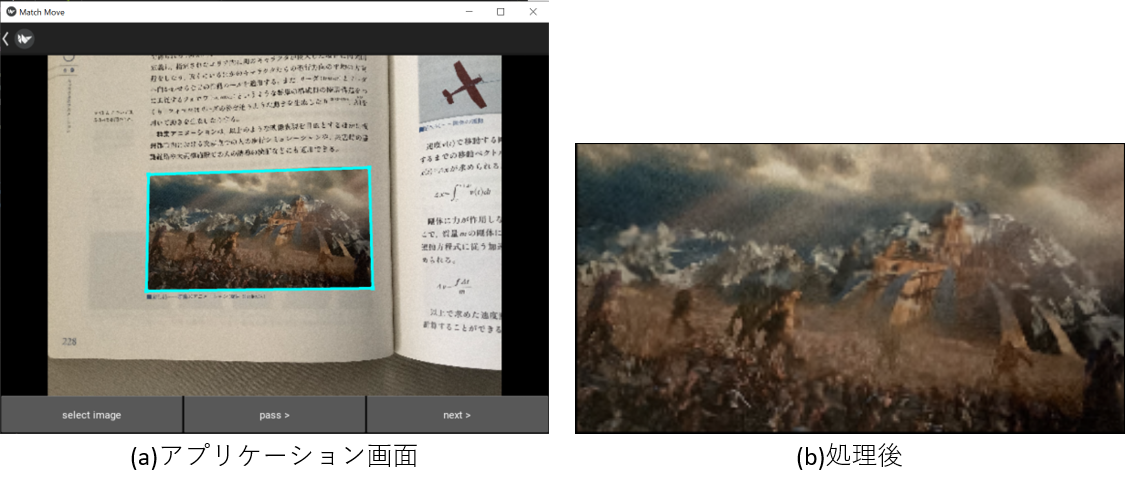
\includegraphics[width=1\linewidth]{fig/clip.png}
    \caption{テンプレート画像のクリッピング}
    \label{fig:clip}
\end{figure}
図\ref{fig:clip}(a)のアプリケーション画面において、
水色のユーザが指定したものであり、
各頂点をクリックすることで選択できるようになっている。
(b)はクリッピングした結果である。
なお変形先については\ref{sec:size}節で述べたように二種類の方法で変形する。

\subsection{テンプレート画像のサイズと精度}\label{sec:size_acc}
本節では\ref{sec:size}節で述べた二種類のサイズとマッチングの精度を比較する。
適用先画像には「target.mov」における1フレーム目を使用する。
また、マッチングアルゴリズムにはSIFTを使用する。
以下にそれぞれにマッチング処理を適用した結果を
図\ref{fig:size_acc_same}及び\ref{fig:size_acc_diff}に示す。

\begin{figure}[h]
    \centering
    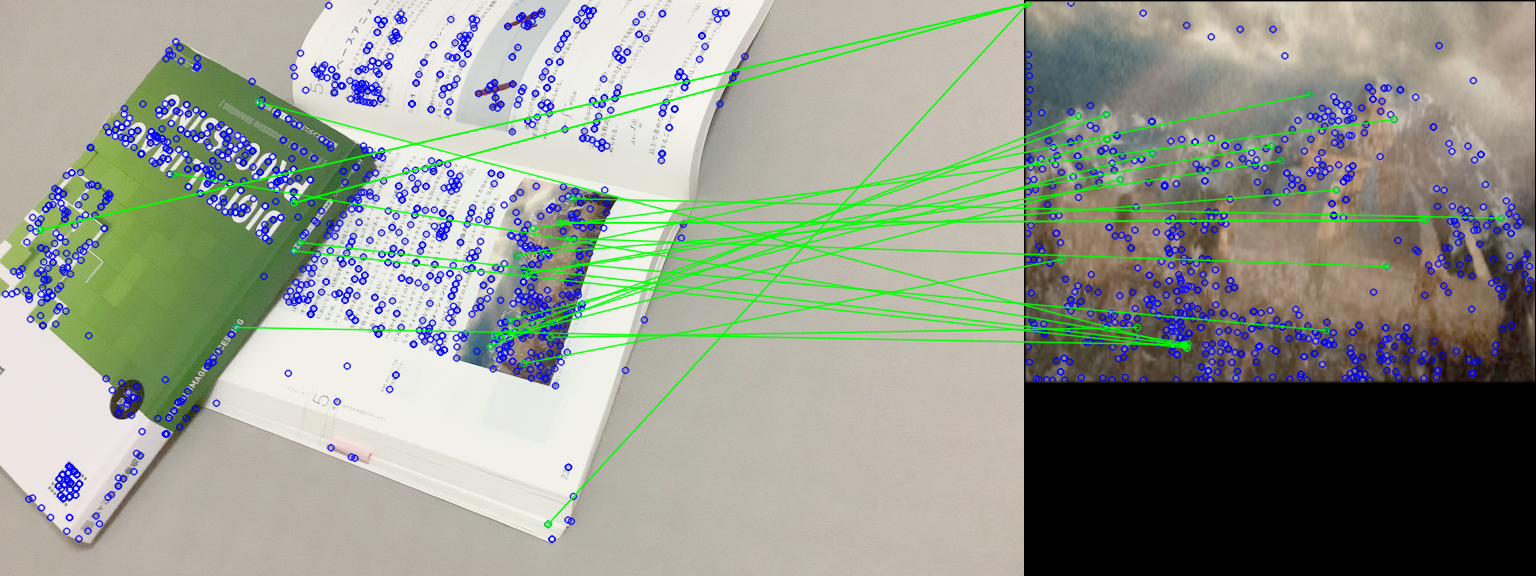
\includegraphics[width=1\linewidth]{fig/matches_SIFT_difference.png}
    \caption{差し替え先画像の高さ・幅に合わせるマッチング}
    \label{fig:size_acc_diff}
\end{figure}

\begin{figure}[h]
    \centering
    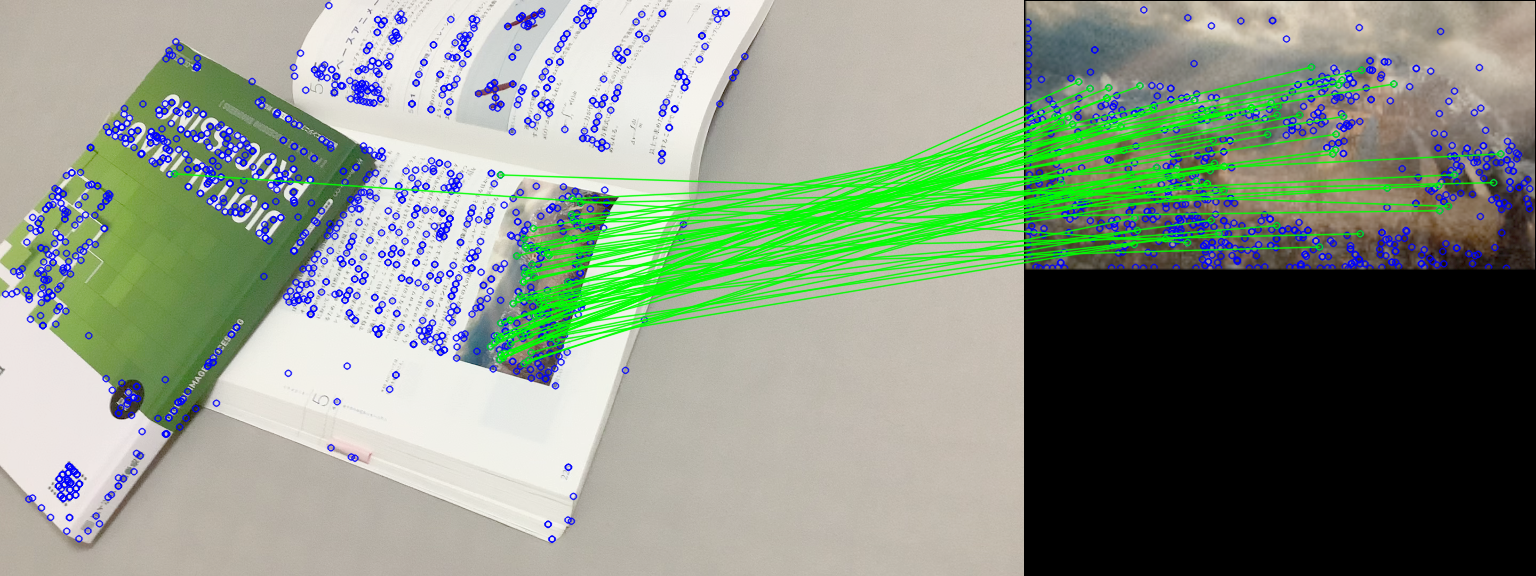
\includegraphics[width=1\linewidth]{fig/matches_SIFT_same.png}
    \caption{テンプレート画像の高さ・幅に合わせるマッチング}
    \label{fig:size_acc_same}
\end{figure}

図\ref{fig:size_acc}及び\ref{fig:size_acc_diff}から分かるように、
アスペクト比を変化させないほうが明らかに検出精度が高いことが分かる。
この図から、マッチング数、ミスマッチ数を数えた結果を表\ref{tb:size_acc}に示す。
なお、ミスマッチ数については正確に数えることが困難であるため、
明らかに適用画像から外れた点のみを数えた。

\begin{table}[h]
    \centering
    \caption{テンプレート画像のサイズと精度}
    \label{tb:size_acc}
    \begin{tabular}{lccc} \hline \hline
         & マッチング数 & ミスマッチ数 & 精度[\%]\\ \hline
        差し替え先画像の高さ・幅に合わせる & 28 & 8 & 71.4 \\
        テンプレート画像の高さ・幅に合わせる & 68 & 2 & 97.1 \\ \hline
    \end{tabular}
\end{table}

表\ref{tb:size_acc}から分かるように、
マッチング数においてもミスマッチ数においても
テンプレート画像の高さ・幅に合わせた方が優れている。
結果として後者の方が高い精度を記録している。

この結果を踏まえて、以降の評価ではテンプレート画像の高さ・幅に画像サイズを合わせて行う。

\subsection{置換精度}
本節では、様々な状況における置換の精度を評価する。
具体的には図\ref{fig:env_data}に示す、
通常の画像、ブレの画像、斜めから見た画像、そして90°の回転を与えた画像
に対して正しく置換できるかを評価する。

\begin{figure}[h]
    \centering
    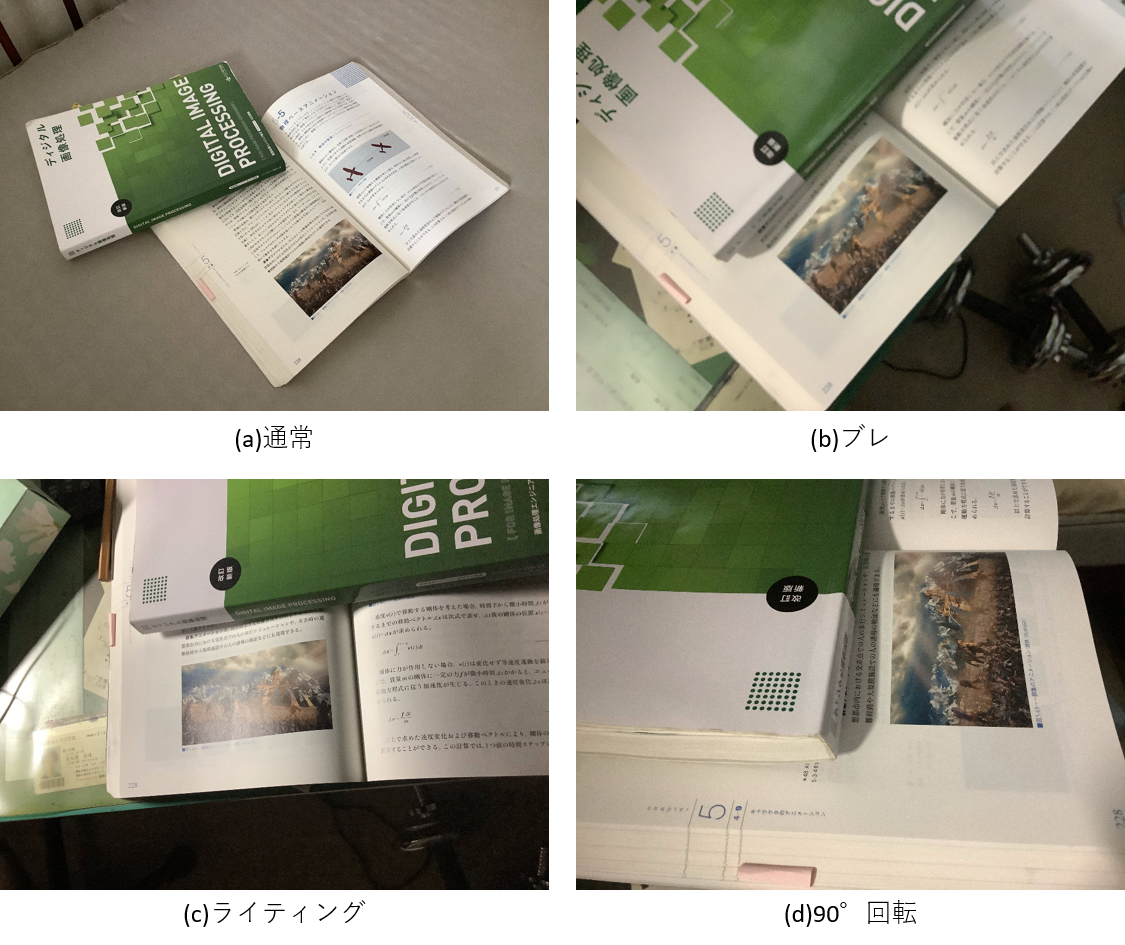
\includegraphics[width=1\linewidth]{fig/env_data.png}
    \caption{環境の異なる各データ}
    \label{fig:env_data}
\end{figure}

この評価は数値で数値で表すことが難しいため、視覚的に比較する。
図\ref{fig:various_env}に実行結果を示す。
\begin{figure}[h]
    \centering
    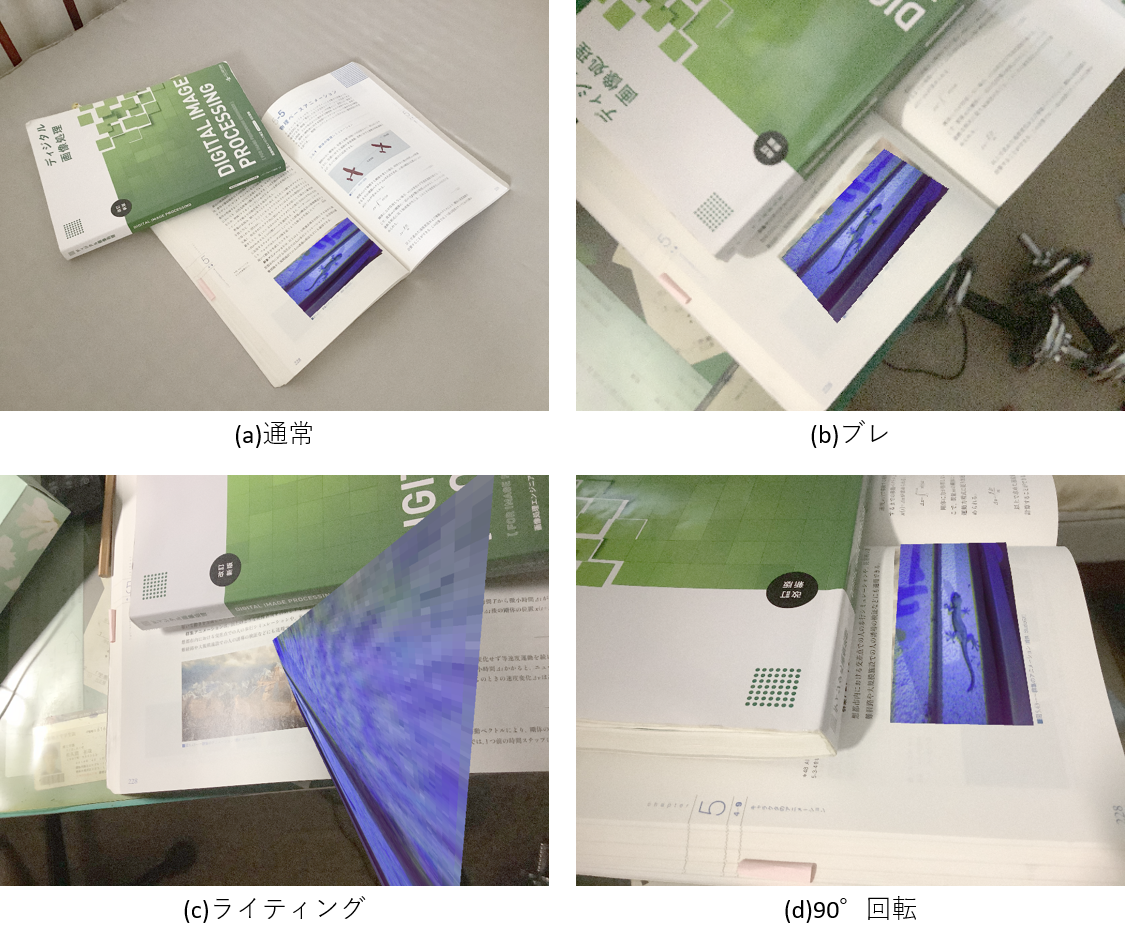
\includegraphics[width=1\linewidth]{fig/env.png}
    \caption{各環境下での置換結果}
    \label{fig:various_env}
\end{figure}
図\ref{fig:various_env}(a)(b)(d)から分かるように、多少のブレや回転に対しては、
ある程度頑健に作用している
また、(a)(b)(d)はどの画像もスケールが異なっているのにもかかわらず、
置換できていることからスケールに対しても頑健であることが分かる。
これは本アプリケーションが特徴量検出アルゴリズムとしてSIFTを採用していることに起因している。
SIFT特徴量はスケールや移動、回転に対して頑健な性質をもつ。
そのために(a)や(d)において問題なくマッチングを行い、置換できたと言える。
また、今回発生したブレは等方向的あることから、
ある種のスケールと捉えられるため、SIFTで上手くマッチングできたと考えられる。
一方で(c)のようにライティングが
変化した際には上手く置換できていないことが分かる。
これは、今回与えたライティングは対象領域を不均一に変化させていることが原因であると
考えらえる。これは画像のテクスチャが変化していることを意味するため、
正しくマッチングを行えなかったと考えられる。

\subsection{部分領域抽出による精度及び速度向上}
本節では\ref{sec:acc_speed}で説明した手法によって、
動画データに対して、精度向上及び速度向上を達成できたかを評価する。
本評価においてソースコード\ref{py:replace2}のradiusは0とした。

表\ref{tb:apply_time}に1フレーム当たりの実行時間を示す。
なお、この評価にはフレームの読み出しから、
置換結果の書き込みまでを含めた全体の時間である。
\begin{table}[h]
    \centering
    \caption{テンプレート画像のサイズと精度}
    \label{tb:apply_time}
    \begin{tabular}{lccc} \hline \hline
         & 実行時間[sec/frame] \\ \hline
        適用前 & 0.287 \\
        適用後 &  0.243 \\ \hline
    \end{tabular}
\end{table}
表\ref{tb:apply_time}から分かるようにアルゴリズムを適用することで、
1フレーム当たりの実行時間は約84.7\%になっている。
本評価で使用した動画は全体で131フレームあるため、
処理時間は5.76秒だけ削減することができた。
アルゴリズムを適用することによって探索領域は約40\%になっており、
その分だけ計算が削減されるが、
実行時間のはそれほど減少しないのは、領域を切り出すために、
ソースコード\ref{py:replace2}の36から48行目のような処理を行う必要があるためであると
考えられる。

精度向上に関しては添付した「result\_before.mp4」「result\_after.mp4」を参照されたい。
精度に関しては一長一短であるように見られる。
適用前の「result\_before.mp4」においては、前半はより安定しているが、
後半にカメラの移動が速くなると、上手く検出できなくなっている一方で、
「result\_after.mp4」は前半の安定感こそ多少劣るものの、
後半の誤差は比較的小さいように思われる。
特に結果が顕著であったフレームを図\ref{fig:apply}に実行結果を示す。

\begin{figure}[h]
    \centering
    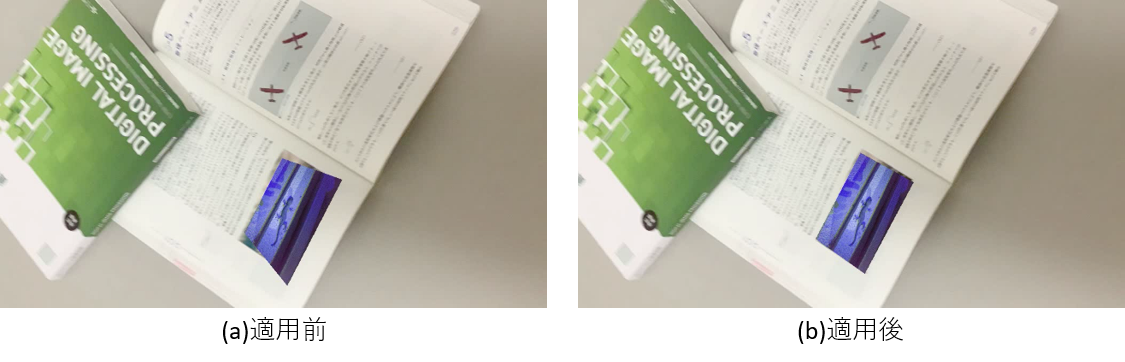
\includegraphics[width=1\linewidth]{fig/apply.png}
    \caption{適用前後で変化が顕著であったフレーム}
    \label{fig:apply}
\end{figure}

図から分かるようにこのフレームは素早くカメラを移動したことにより、
ある方向にブレが生じている。
これによって、適用前の結果では本来対応しているはずの画素同士の類似度が低下し、
誤った対応をとってしまったためであると考えらえる。
適用後の場合は探索領域を絞ったために誤った対応をとる確率が低下し、
比較的上手く置換できたと言える。


% \begin{table}[h]
%     \centering
%     \caption{テンプレート画像のサイズと精度}
%     \label{tb:size_acc}
%     \begin{tabular}{lccc} \hline \hline
%              & target & light
%         通常 & 3.035+106.429+99.911+12.75595792652888
%     \end{tabular}
% \end{table}
\section{結論}\label{sec:conc}
本レポートはスポーツ中継のバーチャル広告などで使用される、
画像の差し替え技術を利用したアプリケーションを作成した。

SIFTを利用した特徴量によって並進・スケール・回転にある程度
頑健に置換できることを示した。
また、動画を対象としているという特徴を活かして、
精度を保つ、あるいは向上させながらも80\%程度の計算時間で実行できた。


今後の展望としては、次のような工夫が考えられる。
\begin{itemize}
    \item 特徴点検出アルゴリズムの検討
    \item 処理の高速化
\end{itemize}

現在の実装ではSIFT特徴量を利用しているが、
このアルゴリズムにはライセンスが必要であり、
商用のアプリケーションとしてリリースするには向いていない。
この問題を解決するアルゴリズムとして、AKAZE\cite{akaze}
などのアルゴリズムが提案されている。
AKAZEは商用利用できるだけでなく、SIFTで使用されている、
スケールスペースではガウシアンフィルタが
等方的に作用するために、エッジもぼやかしてしまうという欠点を
解決できるとされている\cite{akaze}。

また、本実装はPythonを利用しているために、
C++等の低級言語と比較して実行速度に難がある。
この問題を解決するために、
本実装ではできるだけfor文を使用せずに、
テンソル演算を活用した。
テンソル演算を活用できるということは
インデックス間で処理が独立していることを示しており、
GPGPUやOpenMPなどを活用できると言える。



\bibliographystyle{sieicej}
\bibliography{refer}
\end{document}


% アルゴリズム
% 1. 走査対象の画像を切り取る
% 2. 差し替え先の画像を選択
% 3. 差し替え元の動画フレームと対象画像とを特徴点マッチング
% 4. ホモグラフィを計算
% 5. 

% マッチング方法:
%     テンプレートマッチング
%     特徴量マッチング

% 無駄部分のマッチングを省く
%     高速化+精度向上



